\documentclass[aspectratio=169,11pt]{beamer}

\usepackage[T1]{fontenc}
\usepackage[utf8]{inputenc}
\usepackage{lmodern}
\usepackage{graphicx}
\usepackage{booktabs}
\usepackage{tikz}
\usetikzlibrary{arrows.meta,positioning}

\graphicspath{{../figures/}}

\definecolor{snseteal}{HTML}{0E6B5C}
\definecolor{snseblue}{HTML}{1F4E79}
\definecolor{snseamber}{HTML}{D89000}
\definecolor{lightteal}{HTML}{E6F4F1}
\definecolor{lightblue}{HTML}{EAF1F8}
\definecolor{lightamber}{HTML}{FFF4DD}
\definecolor{darkgray}{HTML}{333333}

\usetheme{Madrid}
\usecolortheme[named=snseteal]{structure}
\setbeamertemplate{navigation symbols}{}
\setbeamertemplate{footline}[frame number]

\setbeamercolor{title}{fg=white,bg=snseteal}
\setbeamercolor{frametitle}{fg=white,bg=snseteal}
\setbeamercolor{block title}{fg=white,bg=snseblue}
\setbeamercolor{block body}{fg=darkgray,bg=lightblue}
\setbeamercolor{alertblock title}{fg=white,bg=snseamber}
\setbeamercolor{alertblock body}{fg=darkgray,bg=lightamber}

\title[SnSe Band-Gap Prediction]{Predicting Band Gaps of SnSe-Based Materials from Composition}
\subtitle{Materials Project + matminer + Random Forest}
\author{FDP Capstone Project}
\institute{Machine Learning for Materials and Metallurgical Engineering\\IIT (BHU), UGC MM-TTP}
\date{13--18 July 2026}

\begin{document}

\begin{frame}
  \titlepage
\end{frame}

\begin{frame}{Problem and Motivation}
  \begin{columns}[T,onlytextwidth]
    \column{0.58\textwidth}
    \begin{block}{Project question}
      Can a composition-only model predict whether a Sn--Se-based compound is metal or insulator, and predict the band gap of insulators?
    \end{block}
    \begin{itemize}
      \item SnSe is important for thermoelectric and electronic applications.
      \item Band gap is affected by chemistry, bonding, doping, and structure.
      \item A fast formula-only model can screen candidates before slower calculations or experiments.
    \end{itemize}
    \column{0.38\textwidth}
    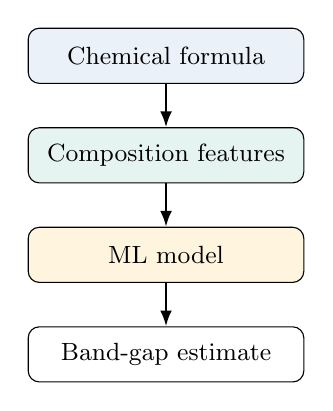
\begin{tikzpicture}[node distance=0.55cm, every node/.style={font=\small}]
      \node[draw,rounded corners,fill=lightblue,minimum width=3.5cm,minimum height=0.7cm] (formula) {Chemical formula};
      \node[draw,rounded corners,fill=lightteal,minimum width=3.5cm,minimum height=0.7cm,below=of formula] (features) {Composition features};
      \node[draw,rounded corners,fill=lightamber,minimum width=3.5cm,minimum height=0.7cm,below=of features] (model) {ML model};
      \node[draw,rounded corners,fill=white,minimum width=3.5cm,minimum height=0.7cm,below=of model] (out) {Band-gap estimate};
      \draw[-{Latex[length=2mm]},thick] (formula) -- (features);
      \draw[-{Latex[length=2mm]},thick] (features) -- (model);
      \draw[-{Latex[length=2mm]},thick] (model) -- (out);
    \end{tikzpicture}
  \end{columns}
\end{frame}

\begin{frame}{Dataset}
  \begin{columns}[T,onlytextwidth]
    \column{0.46\textwidth}
    \begin{block}{Materials Project query}
      \begin{itemize}
        \item Compounds containing Sn and Se.
        \item 220 raw database entries.
        \item 192 unique formulas after cleaning.
        \item Target: computed band gap in eV.
      \end{itemize}
    \end{block}
    \begin{alertblock}{Class balance}
      136 insulators and 56 metals. Accuracy must be compared with this imbalance.
    \end{alertblock}
    \column{0.51\textwidth}
    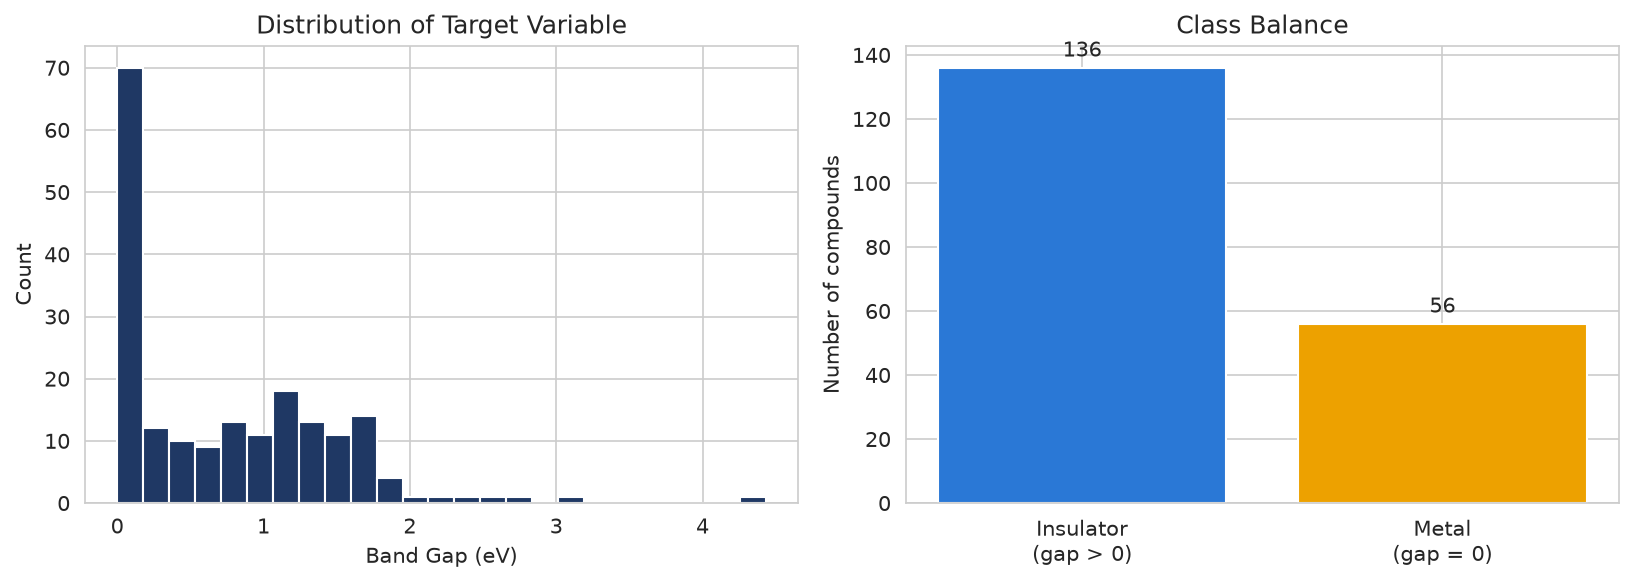
\includegraphics[width=\linewidth]{fig_eda.png}
  \end{columns}
\end{frame}

\begin{frame}{Feature Engineering and Models}
  \begin{columns}[T,onlytextwidth]
    \column{0.50\textwidth}
    \begin{block}{Features}
      \begin{itemize}
        \item Formula parsed with pymatgen.
        \item 132 Magpie descriptors from matminer.
        \item Examples: electronegativity, radius, valence count, periodic column.
        \item No crystal-structure descriptors used.
      \end{itemize}
    \end{block}
    \column{0.47\textwidth}
    \begin{block}{Models}
      \begin{itemize}
        \item Logistic Regression classifier.
        \item Random Forest classifier.
        \item Random Forest regressor for insulators.
        \item Primary evaluation: 5-fold cross-validation.
      \end{itemize}
    \end{block}
  \end{columns}
\end{frame}

\begin{frame}{Results}
  \begin{columns}[T,onlytextwidth]
    \column{0.42\textwidth}
    \small
    \begin{table}
    \centering
    \begin{tabular}{lc}
      \toprule
      Task & Result \\
      \midrule
      RF classification & \(80.2\% \pm 3.7\%\) \\
      Logistic classification & \(78.1\% \pm 6.5\%\) \\
      RF regression MAE & \(0.357 \pm 0.072\) eV \\
      RF regression \(R^2\) & \(0.401 \pm 0.168\) \\
      \bottomrule
    \end{tabular}
    \end{table}
    \normalsize
    \textbf{\color{snseteal}Finding:} Random Forest gives the best screening workflow, but regression is not exact.
    \column{0.55\textwidth}
    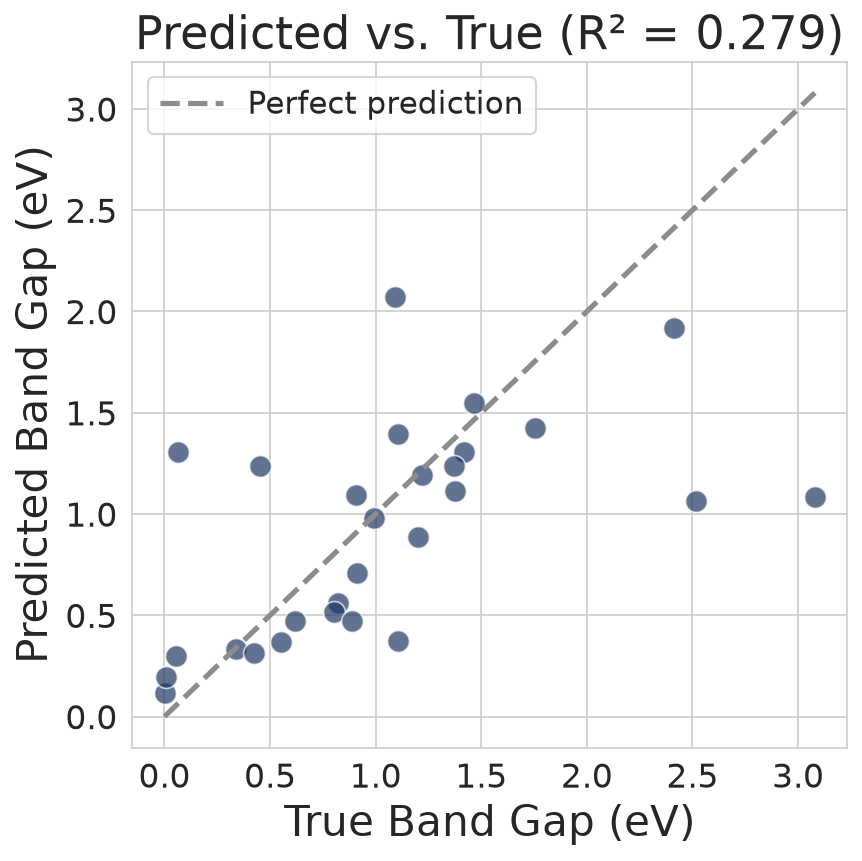
\includegraphics[height=0.68\textheight]{fig_predictions.png}
  \end{columns}
\end{frame}

\begin{frame}{Feature Importance}
  \begin{columns}[T,onlytextwidth]
    \column{0.55\textwidth}
    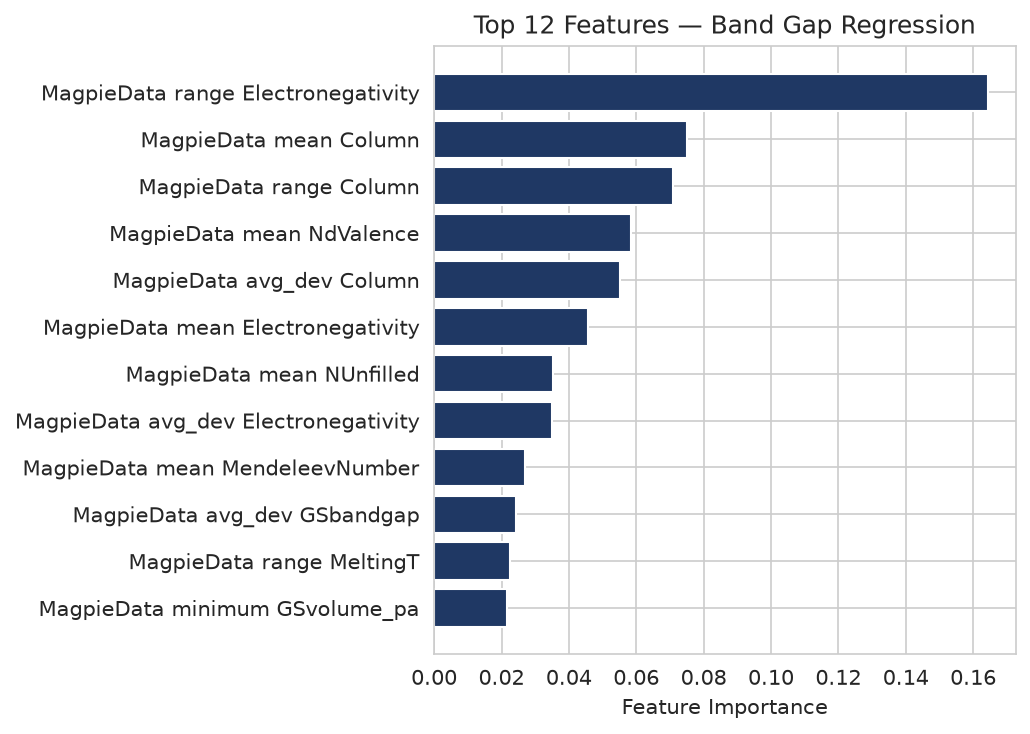
\includegraphics[width=\linewidth]{fig_importance.png}
    \column{0.42\textwidth}
    \begin{block}{Main insight}
      Electronegativity range is the strongest predictor for the band-gap regression model.
    \end{block}
    \begin{itemize}
      \item Large electronegativity contrast changes bonding character.
      \item Bonding character is related to band-gap opening.
      \item Feature importance is predictive evidence, not direct proof of causation.
    \end{itemize}
  \end{columns}
\end{frame}

\begin{frame}{Limitations and Next Steps}
  \begin{columns}[T,onlytextwidth]
    \column{0.48\textwidth}
    \begin{block}{Limitations}
      \begin{itemize}
        \item Formula-only features cannot distinguish polymorphs.
        \item 192 compounds is modest for 132 features.
        \item Class imbalance affects accuracy interpretation.
        \item Target is computed band gap, not experimental band gap.
      \end{itemize}
    \end{block}
    \column{0.48\textwidth}
    \begin{block}{Next steps}
      \begin{itemize}
        \item Add crystal-structure descriptors.
        \item Expand to SnS, SnTe, PbSe, PbTe, GeSe, and related compounds.
        \item Compare more models using repeated cross-validation.
      \end{itemize}
    \end{block}
  \end{columns}
\end{frame}

\begin{frame}{Conclusion}
  \begin{block}{Final message}
    A composition-only Random Forest model gives a useful first-pass screening signal for Sn--Se-based materials, but it should guide candidate selection rather than replace structure-aware calculations or experiments.
  \end{block}
  \vspace{0.4cm}
  \begin{center}
  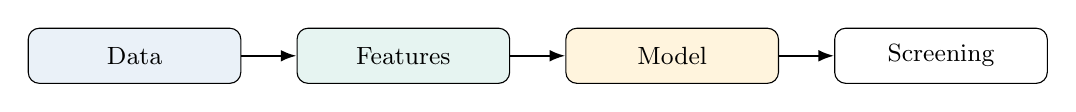
\begin{tikzpicture}[node distance=0.7cm, every node/.style={font=\small}]
    \node[draw,rounded corners,fill=lightblue,minimum width=2.7cm,minimum height=0.7cm] (data) {Data};
    \node[draw,rounded corners,fill=lightteal,minimum width=2.7cm,minimum height=0.7cm,right=of data] (features) {Features};
    \node[draw,rounded corners,fill=lightamber,minimum width=2.7cm,minimum height=0.7cm,right=of features] (model) {Model};
    \node[draw,rounded corners,fill=white,minimum width=2.7cm,minimum height=0.7cm,right=of model] (screen) {Screening};
    \draw[-{Latex[length=2mm]},thick] (data) -- (features);
    \draw[-{Latex[length=2mm]},thick] (features) -- (model);
    \draw[-{Latex[length=2mm]},thick] (model) -- (screen);
  \end{tikzpicture}
  \end{center}
\end{frame}

\end{document}

